\documentclass[14pt, a4paper]{extarticle}
\usepackage{GOST}
\usepackage{array}
\usepackage{verbatim}
\usepackage[detect-all]{siunitx}
\usepackage{amsmath}
\usepackage{amssymb}
\usepackage[utf8]{inputenc}
\usepackage{hyperref}

\usepackage{ifthen}


\usepackage{tempora}


\makeatletter
\renewcommand\@biblabel[1]{#1.}
\makeatother

% Для листинга кода:
\usepackage{listings}
\lstset{ %
	language=python,                 % выбор языка для подсветки (здесь это С)
	basicstyle=\small\sffamily, % размер и начертание шрифта для подсветки кода
	numbers=left,               % где поставить нумерацию строк (слева\справа)
	numberstyle=\tiny,           % размер шрифта для номеров строк
	stepnumber=1,                   % размер шага между двумя номерами строк
	numbersep=5pt,                % как далеко отстоят номера строк от подсвечиваемого кода
	showspaces=false,            % показывать или нет пробелы специальными отступами
	showstringspaces=false,      % показывать или нет пробелы в строках
	showtabs=false,             % показывать или нет табуляцию в строках
	frame=single,              % рисовать рамку вокруг кода
	tabsize=2,                 % размер табуляции по умолчанию равен 2 пробелам
	captionpos=t,              % позиция заголовка вверху [t] или внизу [b] 
	breaklines=true,           % автоматически переносить строки (да\нет)
	breakatwhitespace=false, % переносить строки только если есть пробел
	escapeinside={\#*}{*)}   % если нужно добавить комментарии в коде
}


%для графиков
\usepackage{pgfplots}
\usepackage{filecontents}
\usetikzlibrary{datavisualization}
\usetikzlibrary{datavisualization.formats.functions}

\begin{document}
	
	\begin{table}[ht]
		\centering
		\begin{tabular}{|c|p{400pt}|} 
			\hline
			\begin{tabular}[c]{@{}c@{}} 
\includegraphics[scale=1]{baum.jpg} \\\end{tabular} &
			\footnotesize\begin{tabular}[c]{@{}c@{}}\textbf{Министерство~науки~и~высшего~образования~Российской~Федерации}\\\textbf{Федеральное~государственное~бюджетное~образовательное~учреждение}\\\textbf{~высшего~образования}\\\textbf{«Московский~государственный~технический~университет}\\\textbf{имени~Н.Э.~Баумана}\\\textbf{(национальный~исследовательский~университет)»}\\\textbf{(МГТУ~им.~Н.Э.~Баумана)}\\\end{tabular}  \\
			\hline
		\end{tabular}
	\end{table}
	\noindent\rule{\textwidth}{4pt}
	\noindent\rule[14pt]{\textwidth}{1pt}
	\hfill 
	\noindent
	\makebox{ФАКУЛЬТЕТ~}%
	\makebox[\textwidth][l]{\underline{~«Информатика и системы управления»~~~~~~~~~~~~~~~~~~~~~~~~~~~~~~~~~}}%
	\\
	\noindent
	\makebox{КАФЕДРА~}%
	\makebox[\textwidth][l]{\underline{~«Программное обеспечение ЭВМ и информационные технологии»~}}%
	
	
	\begin{center}
		\vspace{1.5cm}
		{\bf\huge Отчёт\par}
		{\bf\Large по лабораторной работе № 5\par}
		\vspace{0.7cm}
	\end{center}
	
	
	\noindent
	\makebox{\large{\bf Название:}~~~}
	\makebox[\textwidth][l]{\large\underline{Определение вероятности отказа~~~~~~~~}}
	
	\noindent
	\makebox{\large{\bf Дисциплина:}~~~}
	\makebox[\textwidth][l]{\large\underline{~Моделирование~~~~~~~~~~~~~~~~~~~~~~~~~~}}\\
	
	\vspace{1.5cm}
	\noindent
	\begin{tabular}{l c c c c c}
		Студент      & ~ИУ7-75Б~               & \hspace{2.5cm} & \hspace{2cm}                 & &  Д.В. 
		Сусликов \\\cline{2-2}\cline{4-4} \cline{6-6} 
		\hspace{3cm} & {\footnotesize(Группа)} &                & {\footnotesize(Подпись, дата)} & & {\footnotesize(И.О. Фамилия)}
	\end{tabular}
	
	\noindent
	\begin{tabular}{l c c c c}
		Преподаватель & \hspace{5cm}   & \hspace{2cm}                 & & ~~~~~~И.В. Рудаков~~~~~~\\\cline{3-3} \cline{5-5} 
		\hspace{3cm}  &                & {\footnotesize(Подпись, дата)} & & {\footnotesize(И.О. Фамилия)}
	\end{tabular}
	
	\vspace{0.6cm}
	\begin{center}	
		\vfill
		\large \textit {Москва, 2021}
	\end{center}
	
	\thispagestyle {empty}
	\pagebreak
	
	% СОДЕРЖАНИЕ 
	\clearpage
	\tableofcontents
		
	% ВВЕДЕНИЕ
	\clearpage
	\section*{Задание}
	\addcontentsline{toc}{section}{Задание}
	В информационный центр приходят клиенты через интервал времени 10 +- 2 минуты. Если все три имеющихся оператора заняты, клиенту отказывают в обслуживании. Операторы имеют разную производительность и могут обеспечивать обслуживание среднего запроса пользователя за 20 +- 5; 40 +- 10; 40 +- 20. Клиенты стремятся занять свободного оператора с максимальной производительностью. Полученные запросы сдаются в накопитель. Откуда выбираются на обработку. На первый компьютер запросы от 1 и 2-ого операторов, на второй – запросы от 3-его. Время обработки запросов первым и 2-м компьютером равны соответственно 15 и 30 мин. Промоделировать процесс обработки 300 запросов. 
	Для выполнения поставленного задания необходимо создать концептуальную модель в терминах СМО, определить эндогенные и экзогенные переменные и уравнения модели. За единицу системного времени выбрать 0,01 минуты.

	
	\begin{figure}[h!]
		\centering{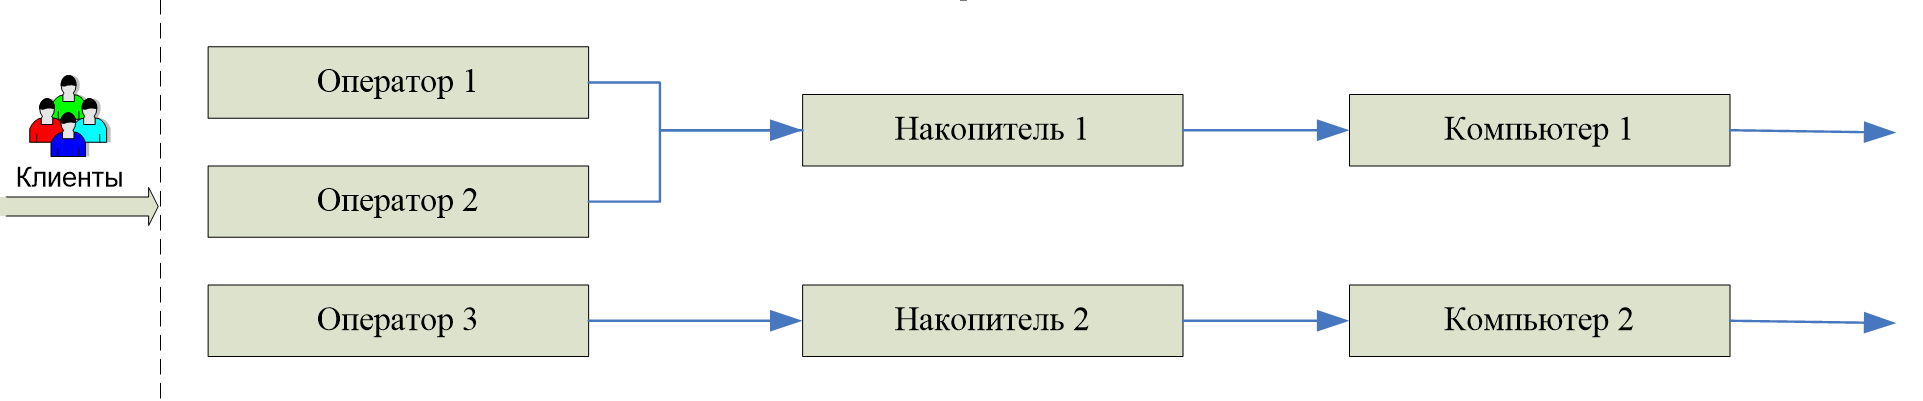
\includegraphics[scale=0.4]{source/task1.png}}
	\end{figure}
	
	\clearpage
	\section*{Аналитическая часть}
	\addcontentsline{toc}{section}{Аналитическая часть}
	В процессе взаимодействия клиентов с информационным центром возможно:
	
	1) Режим нормального обслуживания, т.е. клиент выбирает одного из свободных операторов, отдавая предпочтение тому у которого меньше номер.
	
	2) Режим отказа в обслуживании клиента, когда все операторы заняты. 
	\textbf{Переменные и уравнения имитационной модели }\par
	Эндогенные переменные: время обработки задания i-ым оператором, время решения этого задания j-ым компьютером.
	Экзогенные переменные: число обслуженных клиентов и число клиентов, получивших отказ.
	
	\begin{figure}[h!]
		\centering{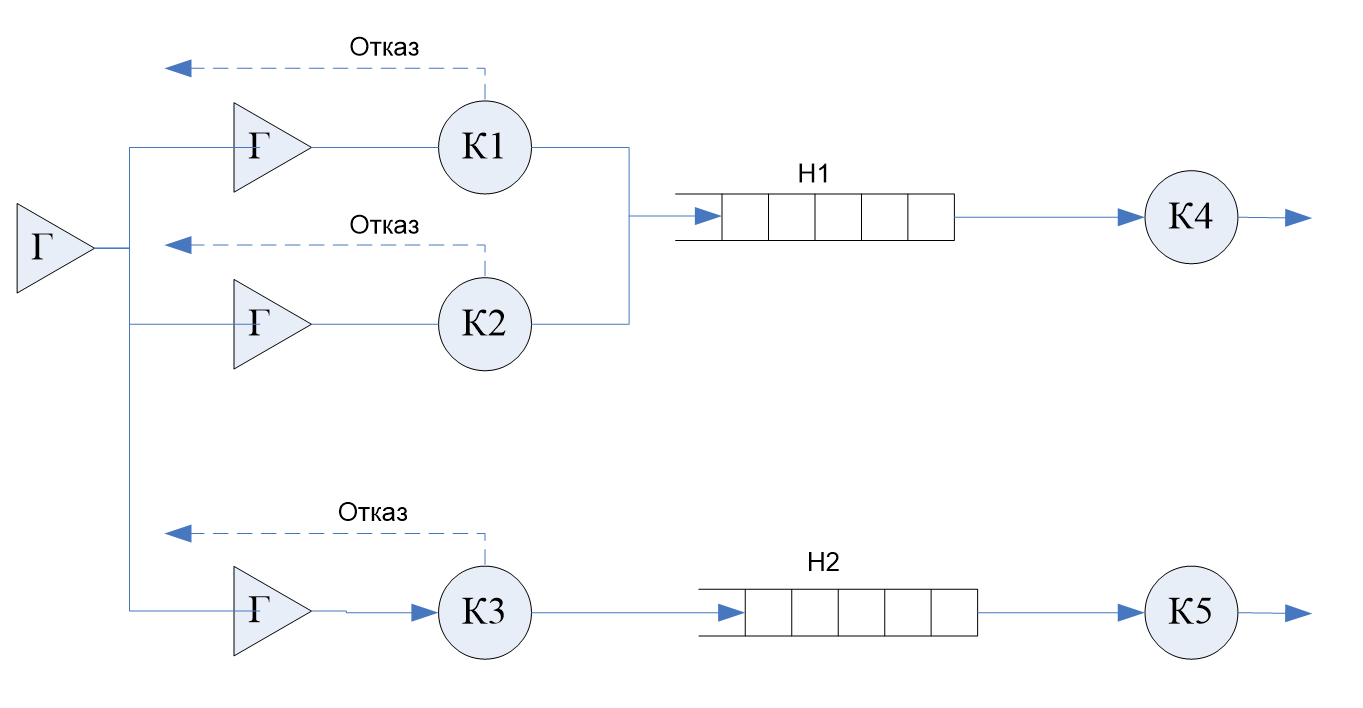
\includegraphics[scale=0.5]{source/task2.png}}
	\end{figure}
	
	\begin{equation*}
		P_{\text{отк}} = \frac{C_{\text{отк}}}{C_{\text{отк}} + C_{\text{обсл}}}
	\end{equation*}
	
	\clearpage
	\section*{Примеры}
	\addcontentsline{toc}{section}{Примеры}
	
	\begin{figure}[h!]
		\centering{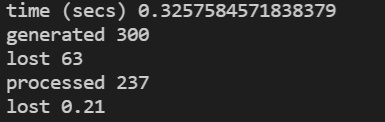
\includegraphics[scale=0.9]{source/1}}
		\centering\caption{300 заявок}
	\end{figure}


	\begin{figure}[h!]
		\centering{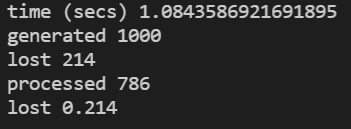
\includegraphics[scale=0.9]{source/2}}
		\centering\caption{1000 заявок}
	\end{figure}
	
	\begin{figure}[h!]
		\centering{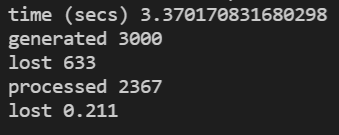
\includegraphics[scale=0.9]{source/3}}
		\centering\caption{3000 заявок}
	\end{figure}
	
	\section*{Вывод}
	\addcontentsline{toc}{section}{Вывод}
	Основываясь на примерах работы системы при 300, 1000 и 3000 заявок, можно сделать вывод, что процент потерь 
	примерно равен 21\%.
	
	
	\clearpage
	\section*{Листинги}
	\addcontentsline{toc}{section}{Листинги}
	
	\begin{lstlisting}[caption=main.py]
		from time import time
		from UniformDistribution import UniformDistribution
		from Generator import Generator
		from Operator import Operator
		from Processor import Processor
		
		timeStep = 0.01 
		
		
		def ChooseOperator(operators):
			for i in range(len(operators)):
				if not operators[i].busy:
					return i
			return -1
		
		def DoStep(generator, operators, processors, requestInfo, newGenerate=True):
			if newGenerate:
				request = generator.UpdateTime(timeStep)
			if request:
				requestInfo['generated'] += 1
				operatorIndex = ChooseOperator(operators)
				if operatorIndex == -1:
					requestInfo['lost'] += 1
				else:
					operators[operatorIndex].acceptRequest(request)
			
			for curOperator in operators:
				curOperator.UpdateTime(timeStep)
			
			for curProcessor in processors:
				res = curProcessor.UpdateTime(timeStep)
				if res == 0:
					requestInfo['processed'] += 1
		
		
		def modeling(generator, operators, processors, incomingRequestAmount):
			requestInfo = {'generated': 0, 'lost': 0, 'processed': 0}
		
			while requestInfo['generated'] < incomingRequestAmount:
				DoStep(generator, operators, processors, requestInfo)
		
			while requestInfo['lost'] + requestInfo['processed'] < incomingRequestAmount:
				DoStep(generator, operators, processors, requestInfo, False)
			
			return requestInfo
		
		
		def main():
			clientGenerator = Generator(UniformDistribution(8, 12))
			
			firstQueue = []
			secondQueue = []
			
			operators = [
				Operator(firstQueue, UniformDistribution(15, 25)),    
				Operator(firstQueue, UniformDistribution(30, 50)),
				Operator(secondQueue, UniformDistribution(20, 60))    
			]
			
			processors = [
				Processor(firstQueue, UniformDistribution(15, 15)),   
				Processor(secondQueue, UniformDistribution(30, 30))   
			]
			
			totalRequests = 3000
			
			tStart = time()
			res = modeling(clientGenerator, operators, processors, totalRequests)
			
			print('time (secs)', time() - tStart)
			for key in res.keys():
			print(key, res[key])
		
		print('lost', res['lost'] / totalRequests)
		
		
		if __name__ == '__main__':
			main()		
	\end{lstlisting}

	\begin{lstlisting}[caption=Generator.py]
	class Generator:
		def __init__(self, distribution):
			self.timeDistribution = distribution
			self.finishTime = 0
			self.requestId = -1
		
		def UpdateTime(self, dt):
			self.finishTime -= dt
		
			if self.finishTime <= 1e-5:
				self.finishTime = self.timeDistribution.generate()
				self.requestId += 1
				return self.requestId
			
			return None	
	\end{lstlisting}
	
	\newpage
	\begin{lstlisting}[caption=Processor.py]
	class Processor:
		def __init__(self, requestsQueue, distribution):
			self.timeDistribution = distribution
			self.busy = False
			self.requestsQueue = requestsQueue
			self.finishTime = 0
		
		def UpdateTime(self, dt):
			self.finishTime -= dt
			
			if self.busy and self.finishTime <= 1e-5:
				self.busy = False
				self.curRequest = None
				return 0
		
			if not self.busy and len(self.requestsQueue) != 0:
				self.requestsQueue.pop(0)
				self.finishTime = self.timeDistribution.generate()
				self.busy = True
				return 1
		
			return 2	
	\end{lstlisting}	

	\begin{lstlisting}[caption=Operator.py]
	class Operator:
		def __init__(self, queue, distribution):
			self.timeDistribution = distribution
			self.busy = False
			self.queue = queue
			self.curRequest = None
			self.finishTime = 0
			
		def acceptRequest(self, request):
			self.busy = True
			self.curRequest = request
			self.finishTime = self.timeDistribution.generate()
		
		def finishCurRequest(self):
			self.queue.append(self.curRequest)
			self.busy = False
			self.curRequest = None
		
		def UpdateTime(self, dt):
			self.finishTime -= dt
			if self.busy and self.finishTime <= 1e-5:
				self.finishCurRequest()
				return 0
			return 2	
	\end{lstlisting}
\end{document}